\chapter{The Bow}\label{ch:bow}
The bow is a very interesting 

as its excitation mechanism is based on friction. 

The bow

Excites the system with a force due to friction, which has a nonlinear relationship to the relative velocity between the bow and the string. 

Helmholtz motion..

\begin{figure}[h]
    \centering
    \begin{tikzpicture}[->,node distance=3cm,
        thick,main node/.style={circle,draw}]
    
        \node[] (image) at (0,0) {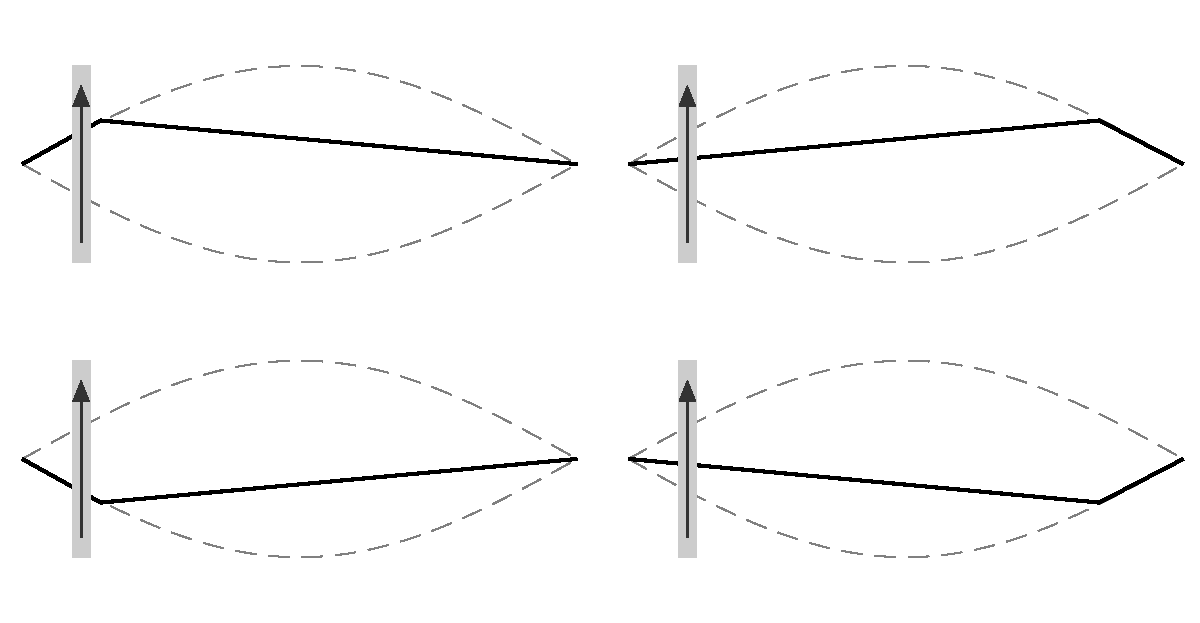
\includegraphics[width=1\columnwidth]{figures/exciters/helmholtz.eps}};
    
        \draw[thick, ->] (-0.25,0.60) arc (110:430:0.6);
        
      \end{tikzpicture}
    \caption{Helmholtz motion. \label{fig:helmholtz}}
\end{figure}

coined as `stick-slip' motion by Bowden and Leben in 1939 \cite{Bowden1939}

See fx. \url{https://www.youtube.com/watch?v=6JeyiM0YNo4}

Characteristic triangular motion (wave shapes?)

The first nonlinear systems in the context of musical instrument simulations, including the bowed string, were presented by McIntyre, et al. in 1983 \cite{McIntyre1983}. The first real-time implementation of the bowed string was due to Smith in 1986 and used digital waveguides for the string and a look-up table for the friction model \cite{Smith1986}. Simultaneously, Florens et al. published a real-time implementation of the bowed string, but instead, the string was modelled using mass-spring systems and the friction model used a static friction model \cite{Florens1986} (see Section \ref{sec:staticFricMod}). 

The first \todo{check with stefania}appearance of FDTD methods in bowed strings was in \cite{Maestre2014}  where these methods were used to implement a thermal friction model proposed by Woodhouse in \cite{Woodhouse2003}. The string, however, was implemented using digital waveguides. Desvages implemented a bowed string model using a static friction model and a two-polarisation FDTD model for the string in \cite{Desvages2016, Desvages2018}.

Before introducing various friction models, a brief introduction on interpolation and spreading operators will be given.


\section{Interpolation and Spreading operators}\label{sec:interpolationSpreading}
By now it must be clear that distributed FD schemes are an approximation to continuous space (and time) using a finite amount of points. If one would like to listen to a location between specified grid points, one can use interpolation. For this end, an \textit{interpolation operator} $I(x_\itxt)$ can be introduced and can be applied to a grid function. This operator is a function of $x_\itxt$, the (continuous) location of interest and can be defined in various levels of accuracy.

The simplest interpolation operator is of '0\textsuperscript{th}'-order and is defined as
\begin{equation}\label{eq:zerothOrderI}
    I_0(x_\itxt) = \begin{cases}
        1, & \text{if}\ l = l_\itxt,\\
        0, & \text{otherwise},
    \end{cases}
\end{equation}
where the grid location of interest is defined as $l_\itxt = \floor[x_\itxt / h]$. See Figure \ref{fig:zerothOrderInterpol}. Instead of actually performing an interpolation operation, $I_0$ simply floors its input to the grid location below. As an example, for a 1D system of length $L=1$ described by $u(x,t)$, the location of interest is at $x_\itxt = 0.25$. If the grid spacing $h = 0.2$ the grid point of interest will be $l_\itxt = \floor[0.25/0.2] = \floor[1.25] = 1$. Writing this in operator form yields
\begin{equation*}
    u(0.25, t)\approxeq I_0(0.25)\uln = u_1^n.
\end{equation*}

% \input{exciters/interpolation.tex}


A slightly more accurate way to perform 0\thOrder interpolation is to round $x_\itxt/h$ to the nearest neighbour, rather than using the flooring operation. 

First-order or linear interpolation also uses the fractional part of the flooring operation according to $\alpha_\itxt = x_\itxt / h - l_\itxt$ and is defined as
\begin{equation}\label{eq:firstOrderI}
    I_1(x_\itxt) = \begin{cases}
        (1-\alpha_\itxt), & \text{if}\ l = l_\itxt,\\
        \alpha_\itxt , & \text{if}\ l = l_\itxt + 1,\\
        0 & \text{otherwise.}
    \end{cases}
\end{equation}
See Figure \ref{fig:firstOrderInterpol}. When applied to a grid function, all multiplications get added to obtain the interpolated value. Using the same example as before, $\alpha = 1.25 - \floor[1.25] = 0.25$ and
\begin{equation*}
    u(0.25, t)\approxeq I_1(0.25)\uln = 0.75u_1^n + 0.25 u_2^n,
\end{equation*}

The highest order interpolator used in this project is the Lagrange cubic interpolator: 
\begin{equation}\label{eq:cubicI}
    I_3(x_\itxt) = \begin{cases}
        -\alpha_\itxt (\alpha_\itxt-1)(\alpha_\itxt-2)/6, & l = l_\itxt-1,\\
        (\alpha_\itxt-1)(\alpha_\itxt+1)(\alpha_\itxt-2)/2,  & l = l_\itxt,\\
        -\alpha_\itxt (\alpha_\itxt+1)(\alpha_\itxt-2)/2, & l = l_\itxt + 1,\\
        \alpha_\itxt (\alpha_\itxt+1)(\alpha_\itxt-1)/6, & l = l_\itxt + 2,\\
        0, & \text{otherwise.}
    \end{cases}
\end{equation}
See Figure \ref{fig:cubicInterpol}. One could potentially create higher-order interpolation operators, but as one is restricted to a finite domain, the flexibility of the implementation will become less. Notice that if $\alpha_\itxt = 0$, the higher-order interpolators reduce to the $0$\thOrder one in Eq. \eqref{eq:zerothOrderI}.

\def\figWidth{0.32}
\begin{figure}[h]
    \centering
    \subfloat[$0$\thOrder interpolation.\label{fig:zerothOrderInterpol}]{\includegraphics[width=\figWidth\textwidth]{figures/exciters/noInterpol.pdf}}\hfill
    \subfloat[Linear interpolation.\label{fig:firstOrderInterpol}]{\includegraphics[width=\figWidth\textwidth]{figures/exciters/linearInterpol.pdf}}\hfill
    \subfloat[Cubic interpolation.\label{fig:cubicInterpol}]{\includegraphics[width=\figWidth\textwidth]{figures/exciters/cubicInterpol.pdf}}
    \caption{Interpolation with varying orders of accuracy.\label{fig:interpolation}}
\end{figure}

Apart form interpolation operators, one may define \textit{spreading operators} which can be interpreted as an inverse interpolation. A spreading operator $J(x_\itxt)$ is used to interact with a distributed FD scheme in the form of an excitation or other interactions such as connections or collisions between multiple schemes (see Part \ref{part:interactions}).

The spreading operators can be defined in the same way as the interpolation operators described above, yielding a $0$\thOrder spreading operator
\begin{equation}\label{eq:zerothOrderJ}
    J_0(x_\itxt) = \frac{1}{h}\begin{cases}
        1, & \text{if}\ l = l_\itxt,\\
        0, & \text{otherwise},
    \end{cases}
\end{equation}
a linear spreading operator
\begin{equation}\label{eq:firstOrderJ}
    J_1(x_\itxt) = \frac{1}{h}\begin{cases}
        (1-\alpha_\itxt), & \text{if}\ l = l_\itxt,\\
        \alpha_\itxt , & \text{if}\ l = l_\itxt + 1,\\
        0 & \text{otherwise,}
    \end{cases}
\end{equation}
and a Lagrange cubic spreading operator
\begin{equation}\label{eq:cubicJ}
    J_3(x_\itxt) = \frac{1}{h}\begin{cases}
        -\alpha_\itxt (\alpha_\itxt-1)(\alpha_\itxt-2)/6, & l = l_\itxt-1,\\
        (\alpha_\itxt-1)(\alpha_\itxt+1)(\alpha_\itxt-2)/2,  & l = l_\itxt,\\
        -\alpha_\itxt (\alpha_\itxt+1)(\alpha_\itxt-2)/2, & l = l_\itxt + 1,\\
        \alpha_\itxt (\alpha_\itxt+1)(\alpha_\itxt-1)/6, & l = l_\itxt + 2,\\
        0, & \text{otherwise.}
    \end{cases}
\end{equation}
Notice the scaling by $1/h$ which will be more elaborated on in Chapter \ref{ch:connections}. As is the case with the interpolation operators, higher-order spreading operators reduce to Eq. \eqref{eq:zerothOrderJ} if $\alpha_\itxt = 0$.

The spreading operators, $J(x_\itxt)$ approximate the spatial Dirac delta function $\delta(x-x_\itxt)$, a test function defined as
\begin{equation}\label{eq:spatialDirac}
    \delta(x)= \begin{cases}
        \infty, & x = 0,\\
        0, & \text{otherwise},
    \end{cases} \qaq \int_{-\infty}^{\infty} \delta(x)dx = 1,
\end{equation}
used in continuous time to locate an external force to a location $x_\itxt$ along a system distributed over space $x$. Note that the definition in \eqref{eq:spatialDirac} will not be used in practice. Instead, it can be approximated using spreading operators. 

Finally, the following identity is extremely useful when solving systems including interpolation and spreading operators
\begin{equation}\label{eq:identityIJ}
    \langle f, J_o(x_\itxt) \rangle_\D = I_o(x_\itxt) f,
\end{equation}
for any (grid) function $f$ and $I$ and $J$ are of the same order $o$. From this follows, taking the norm of a spreading operator $J_o(x_\itxt)$ over a given domain (see Eq. \eqref{eq:discInnerProd}) is identical to applying to its `dual' interpolation operator (of the same order $o$ and same input $x_\itxt$):
\begin{equation}
    \langle  J_o(x_\itxt), J_o(x_\itxt)\rangle_\D = \lVert J_o(x_\itxt)\rVert^2_\D = I_o(x_\itxt)J_o(x_\itxt).
\end{equation}



\section{The Newton-Raphson Method}\label{sec:newtonRaphson}
Before moving on to more complex excitation mechanisms, it is useful to go over the process of how to solve some of these. 

If a function can not be solved explicitly, due to the presence of a nonlinear dependence on a variable \todo{different wording here} for example, an iterative root-finding method can be used that attempts to find the solution. One option is to use the Newton-Raphson method (or Newton's method for short). For a continuous and differentiable function $f(x) = 0$ its root near can be found
\begin{equation}\label{eq:newtonRaphson}
    x_{i+1} = x_i - \frac{f(x_i)}{f'(x_i)}\ ,
\end{equation}
where the tick is used to denote a derivation with respect to $x$.
This iteration will then be carried out until the difference between the values of two consecutive iterations is smaller than a given threshold:
\begin{equation}\label{eq:NRthreshold}
    |x_{i+1} - x_i| < \epsilon,
\end{equation} 
where $\epsilon$ is a small value, but depends on the situation at hand. To prevent Newton's method from iterating endlessly (which can happen in some cases), one can put a cap on the number of iterations allowed. 

Preferably, the starting point of the iteration, $x_0$, should be close to the value of where the root is expected to be. This is especially the case for a higher-ordered function with multiple roots or multiple local minima, local maxima and inflexion points. 

Algorithm \ref{alg:NR} shows an example of an implementation of the Newton-Raphson method using $f(x) = e^x -1\ \Rightarrow\ f'(x) = e^x $.

\setlstMAT
\begin{lstlisting}[caption={Example of an implementation of the Newton-Raphson method using $f(x) = e^{x} - 1$.}, label=alg:NR]
% An example of the Newton Raphson method using f(x) = exp(x) - 1

x = 1;          % starting point
eps = 1e-4;     % threshold

% if the threshold has not been crossed before this amount of iterations, do not iterate more
maxIterations = 100;    
    
% loop until a maximum number of iterations
for i = 1:maxIterations

    % calculate next iteration (Eq. %*\eqrefMatlab[eq:newtonRaphson]*)
    xNext = x - (exp(x) - 1) / (exp(x));

    % threshold check (Eq. %*\eqrefMatlab[eq:NRthreshold]*)
    if abs(xNext - x) < eps 
        break; % break out of the for loop
    end

    % update the value of x
    x = xNext;
end
disp("The root of f(x) is at x = " + xNext)
\end{lstlisting}

\subsection{Multivariate Newton-Raphson}\label{sec:multivariateNR}
For $M$ functions $f_m$ dependent on $M$ independent variables $x_m$ with $m = \{1, \hdots, M\}$, the Newton-Raphson method can be extended to the following:
\begin{equation}\label{eq:multivariateNR}
    \mathbf{x}_{i+1} = 
    \mathbf{x}_i - 
    \begin{bmatrix}
        \frac{\partial f_1(\mathbf{x}_i)}{\partial x_1} & \hdots & \frac{\partial f_1(\mathbf{x}_i)}{\partial x_M}\\
        \vdots & \ddots & \vdots\\
        \frac{\partial f_M(\mathbf{x}_i)}{\partial x_1} & \hdots & \frac{\partial f_M(\mathbf{x}_i)}{\partial x_M}
    \end{bmatrix}^{-1}
    \begin{bmatrix}
        f_1(\mathbf{x}_i)\\
        \vdots\\
        f_M(\mathbf{x}_i)
    \end{bmatrix},
\end{equation}
where the independent variables are collected in a column vector
\begin{equation}
    \mathbf{x} = \begin{bmatrix}
        x_1\\
        \vdots\\
        x_M
    \end{bmatrix}.
\end{equation}
The matrix in \eqref{eq:multivariateNR} is referred to as the \textit{Jacobian matrix} $\mathbf{J}$ and contains the derivatives of all functions with respect to each individual independent variable. 

As an example, consider the following functions\footnote{Taken from \url{http://fourier.eng.hmc.edu/e176/lectures/NM/node21.html}}:
\begin{align}
    f_1(\mathbf{x}) &= 3 x_1 - \cos(x_2x_3) - 3/2 = 0,\\
    f_2(\mathbf{x}) &= 4x_1^2 - 625 x_2^2 + 2x_3-1 = 0,\\
    f_3(\mathbf{x}) &= 20 x_3 + e^{-x_1x_2}+9 = 0.
\end{align} 
The Jacobian matrix will be 
\begin{equation*}
    \mathbf{J}(\mathbf{x}) = \begin{bmatrix}
        3 & x_3 \sin (x_2x_3) & x_2 \sin(x_2x_3)\\
        8x_1 & -1250 x_2 & 2\\
        -x_2e^{-x_1x_2} & -x_1e^{-x_1x_2} & 20
    \end{bmatrix},
\end{equation*}
and its roots can be found by iteratively calculating Eq. \eqref{eq:multivariateNR} .

\section{Static Friction Models}\label{sec:staticFricMod}
A friction model is a nonlinear function that is (at least) dependent on the relative velocity $\vrel$ between the bow and the string. This function scales how much the bow force affects the bowed object. 
In static friction models, the friction force is defined as a function of this relative velocity only.
The first mathematical description of friction was proposed by Coulomb in 1773 \cite{Coulomb1773}\todo{check references here} to which static friction, or \textit{stiction}, was added by Morin in 1833 \cite{Morin1833} and viscous friction, or velocity-dependent friction, by Reynolds in 1886 \cite{Reynolds1886}. In 1902, Stribeck found a smooth transition between the static and the coulomb part of the friction curve now referred to as the Stribeck effect \cite{Stribeck1902}. The latter is still the standard for static friction models today.

In this project, only the following static friction model has been used \cite{theBible}
\begin{equation}\label{eq:staticFriction}
    \Phi (\vrel) = \sqrt{2a}\vrel e^{-a\vrel^2 + 1/2}.
\end{equation}
See Figure \ref{fig:frictionCharacteristic}. Consider a string, its transverse displacement described by $u(x,t)$ defined for $x\in \D$ (see Chapter \ref{ch:stiffString}). The relative velocity between the string at bow position $x_\Btxt = x_\Btxt(t) \in \D$ and the bow is described as
\begin{equation}\label{eq:vrel}
    \vrel = \pt u(x_\Btxt, t) - v_\Btxt(t)
\end{equation}
(in m/s) with bow velocity $v_\Btxt = v_\Btxt(t)$ (in m/s).

\todo{FULL DOC SWEEP: check figure centering}\begin{figure}[h]
    \centering
    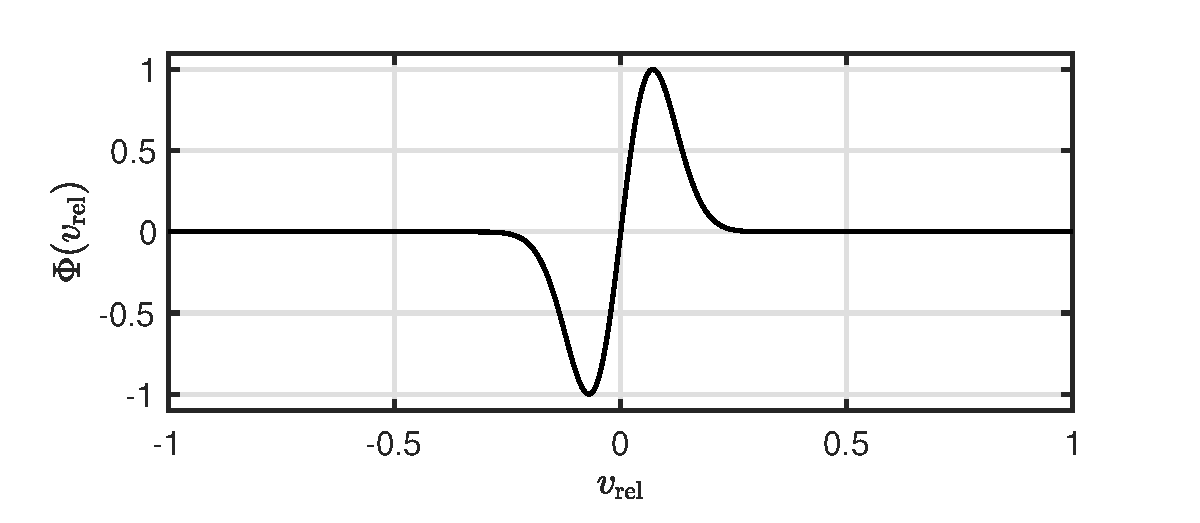
\includegraphics[width=0.8\textwidth]{figures/exciters/frictionCharacteristic.eps}
    \caption{The friction model in \eqref{eq:staticFriction} with $a = 100$. \label{fig:frictionCharacteristic}}
\end{figure}

Many of the friction models contain a discontinuity where the relative velocity $\vrel = 0$ due to a multiplication with $\text{sign}(\vrel)$ in their definition. Equation \eqref{eq:staticFriction} approximates discontinuous bow models using a continuous and differentiable function. This makes it easier to work with when trying to implement the system as will be explained next.

\subsection{The bowed stiff string}
Recalling the PDE of the stiff string in Eq. \eqref{eq:stiffStringPDE}
\begin{equation}
    \rho A \ptt u = T \pxx u - EI \pxxxx u - 2 \sz \rho A \pt u + 2 \so \rho A\pt \pxx u,
\end{equation}
one can add the bow force to the equation according to 
\begin{equation}\label{eq:bowedStiffStringPDE}
    \rho A \ptt u = T \pxx u - EI \pxxxx u - 2 \sz \rho A \pt u + 2 \so \rho A\pt \pxx u - \delta(x-x_\Btxt)f_\Btxt\Phi(\vrel)
\end{equation}
where spatial Dirac delta function $\delta(x-x_\Btxt)$ (in m$^{-1}$) (see Section \ref{sec:interpolationSpreading}) positions the bow along the string and $f_\Btxt = f_\Btxt(t)$ is the bow force (in N). 

\subsubsection{Intuition}
From Eq. \eqref{eq:bowedStiffStringPDE} it can be seen that the bow force gets scaled by the friction model $\Phi(\vrel)$ shown in Figure \ref{fig:frictionCharacteristic}. 
The figure shows that if $\vrel$ is too large (either positively or negatively) the bow term in \eqref{eq:bowedStiffStringPDE} becomes $0$. If, on the other hand, $\vrel$ is closer to $0$, the bow will have an effect on the string. This can be interpreted in terms of static and dynamic friction\footnote{`Static' and `dynamic' friction are unrelated to `static' and `dynamic' friction models.}. A stationary object requires more force to be moved than a moving object, i.e., the static friction coefficient is always higher than the dynamic friction coefficient. This is essentially what the friction model tries to simulate.

\subsubsection{Discrete time}
We continue to discretise \eqref{eq:bowedStiffStringPDE}. Dividing all terms by $\rho A$ and discretising the system yields
%
\begin{equation}\label{eq:bowedStiffStringFDS}
    \dtt \uln = c^2 \dxx \uln - \kappa^2 \dxxxx \uln - 2 \sz \dtd \uln + 2 \so\dtm\dxx \uln - J(x_\Btxt^n)F_\Btxt^n\Phi(\vrel^n),
\end{equation}
with $F_\Btxt^n = f_\Btxt^n/\rho A$ and spreading operator $J(x_\Btxt)$ (in m$^{-1}$) as described in \ref{sec:interpolationSpreading}, the order of which remains undetermined for now. Notice that, as the bow position, bow velocity and bow force are time-dependent, these have received a superscript $n$. These parameters are called control parameters and will be supplied by the performer in the eventual implementation.

The relative velocity in Eq. \eqref{eq:vrel} is discretised using a centred difference operator according to
\begin{equation}\label{eq:vrelDisc}
    \vrel^n = I(x_\Btxt^n)\dtd \uln - v_\Btxt^n.
\end{equation}
The main issue with Eq. \eqref{eq:vrelDisc} is that, due to the centred difference operator, the FD scheme is now nonlinearly dependent on $u_l^{n+1}$. To solve Eq. \eqref{eq:bowedStiffStringFDS}, an iterative solver is required, such as the Newton-Raphson described in Section \ref{sec:newtonRaphson}. This process could be circumvented by using a backward  difference operator in Eq. \eqref{eq:vrelDisc}, but this will affect accuracy of the bow model.

\subsubsection{Solution}
To find a solution for $u_l^{n+1}$ at the bow location, an inner product of the scheme in Eq. \eqref{eq:bowedStiffStringFDS} with spreading operator $J(x_\Btxt^n)$ must be taken which isolates the scheme at the bowing location. Performing this operation and using identity \eqref{eq:identityIJ} yields
\begin{equation}\label{eq:bowLocFDS}
    \begin{aligned}
    I(x_\Btxt^n)\dtt\uln =\ &c^2 I(x_\Btxt^n)\dxx \uln - \kappa^2 I(x_\Btxt^n)\dxxxx \uln- 2 \sz I(x_\Btxt^n)\dtd \uln\\
    & + 2 \so I(x_\Btxt^n)\dtm\dxx \uln - \lVert J(x_\Btxt^n)\rVert^2_\D F_\Btxt^n\Phi(\vrel^n).
    \end{aligned}
\end{equation}
One can rewrite Eq. \eqref{eq:vrelDisc} to 
\begin{equation}
   I(x_\Btxt^n)\dtd \uln =  \vrel^n + v_\Btxt^n,
\end{equation}
and using identity \eqref{eq:identity1}, Eq. \eqref{eq:bowLocFDS} can be rewritten and assigned to a function $g(\vrel^n)$ 
\begin{equation}\label{eq:staticFrictionNRfunc}
    g(\vrel^n) = \left(\frac{2}{k} + 2\sz\right)\vrel^n + \lVert J(x_\Btxt^n)\rVert^2_\D F_\Btxt^n\Phi(\vrel^n) + b^n = 0,
\end{equation}
% Here, $b$ contains all terms not dependent on $\vrel$. As the operators can be interchanged, i.e., the order of application does not matter, could write $b$ according to
where the terms not dependent on $\vrel$ are collected in
\begin{align*}
    b^n =\ &-\frac{2}{k}I(x_\Btxt^n)\dtm \uln-c^2 I(x_\Btxt^n)\dxx \uln + \kappa^2 I(x_\Btxt^n)\dxxxx \uln \\
    &+ \left( \frac{2}{k} + 2 \sz \right)v_\Btxt^n - 2 \so I(x_\Btxt^n)\dtm\dxx \uln.
    % b =&\ \left(-\frac{2}{k}\dtm -c^2 \dxx+ \kappa^2\dxxxx - 2 \so \dtm\dxx\right) I(x_\Btxt^n)\uln + \left( \frac{2}{k} + 2 \sz \right)v_\Btxt^n.
\end{align*}

One can then perform the Newton-Raphson method detailed in Section \ref{sec:newtonRaphson} to iteratively solve for $\vrel$ 

\begin{equation}
    (\vrel^n)_{i+1} = (\vrel^n)_i - \frac{g((\vrel^n)_i)}{g'((\vrel^n)_i)}\ ,
\end{equation}
where
\begin{equation}
    g'(\vrel^n) = \frac{2}{k} + 2\sz + \lVert J(x_\Btxt^n)\rVert^2_\D F_\Btxt^n\Phi'(\vrel^n),
\end{equation}
and 
\begin{equation*}
    \begin{aligned}
        \Phi'(\vrel^n) %&= \sqrt{2a}e^{-a(\vrel^n)^2 + 1/2} + \sqrt{2a}\vrel^n * (-2a\vrel^n)e^{-a(\vrel^n)^2 + 1/2}\\
        %&
        = \sqrt{2a}\left(1 - 2a(\vrel^n)^2\right)e^{-a(\vrel^n)^2+1/2}.
    \end{aligned}
\end{equation*}
\subsubsection{Implementation}
$\epsilon = 10^{-4}$

\begin{equation}
    I(x_\Btxt^n) \dxx \uln = (1-\alpha)\dxx u_{l_\Btxt}^n + \alpha \dxx u_{l_\Btxt+1}^n
\end{equation}

\section{Dynamic Friction Models}
As opposed to less complex static friction models, dynamic friction models relate the relative velocity to the friction force using a differential equation. Dynamic friction models exhibit a phenomenon called \textit{hysteresis}, which is the dependence of a system on its history. 

The first dynamic friction model was due to Dahl \cite{Dahl1968} and captured hysteresis effects. The Stribeck effect was, however, not taken into account. The LuGre model (named after the collaboration between Lund and Grenoble) was then proposed by Canudas de Wit et al. in \cite{Canudas1993, Canudas1995} and extended the Dahl model to take the Stribeck effect into account. The model assumes a large ensemble of bristles between the two sliding surfaces, each of which contributes a tiny amount to the total friction force. The drawback of this model is that it exhibits drift for extremely small external forces. In \cite{Dupont2002}, Dupont et al. extended the LuGre model by allowing for a purely elastic regime that solves the drift issue. This model is referred to as the \textit{elasto-plastic} friction model and is used in this project.

\subsection{The Elasto-Plastic friction model}
In a musical context, the elasto-plastic friction has been thoroughly investigated by Serafin et al. in \cite{Serafin2003, Serafin2004, Avanzini2005}. Like the LuGre model, the elasto-plastic friction model assumes that the friction between the bow and the string is caused by a large quantity of bristles, each of which contributes to the total amount of friction. See Figure \ref{fig:elastoPlastic}.

\begin{figure}[ht]
    \centering
    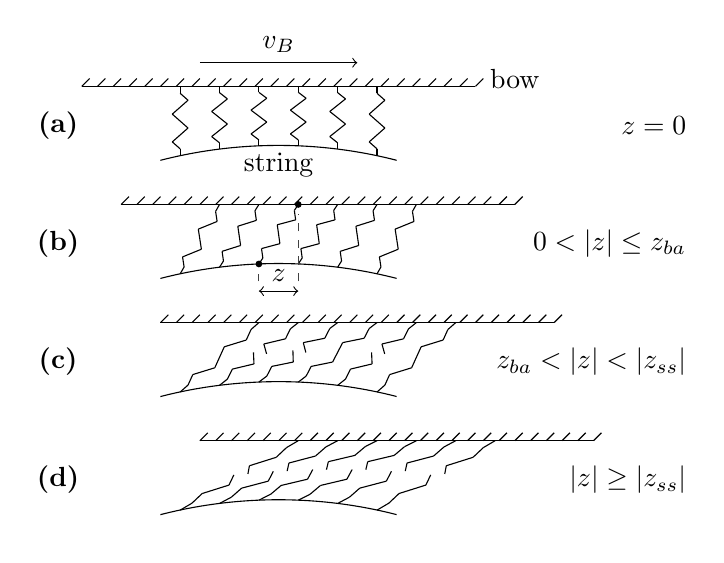
\begin{tikzpicture}
    
    \def\radius{6}; % Radius of the string (>2!)
    \pgfmathsetmacro{\reps}{3}; % How may back-and-forths in the drawing of the springs
    \def\horShift{0.5}; %how far the bow is shifted to the right in b)
    \def\bowSpacing{0.2};
    \def\drawingSpacing{1.5}
    \def\bowWidth{5};
    
    %subfigure letters
    \node (A) at (-2.8, 0.5) {\textbf{(a)}};
    \node (B) at (-2.8, 0.5 - \drawingSpacing) {\textbf{(b)}};
    \node (C) at (-2.8, 0.5 - \drawingSpacing * 2) {\textbf{(c)}};
    \node (D) at (-2.8, 0.5 - \drawingSpacing * 3) {\textbf{(d)}};
    
    %bow velocity arrow
    \draw[->] (-1, 1.3) -- (1, 1.3) node [midway, above] (velText) {$v_\text{B}$};
    
    \pgfmathsetmacro{\zCoordTop}{0};
    \pgfmathsetmacro{\zYCoordBottom}{0};
    \def\springForZ{2}
    \foreach \drawing in {0, ..., 3}
    {
        %% Draw String
        \begin{scope}
            \clip (-1.5,-0.2- \drawing * \drawingSpacing) rectangle (1.5,1.5);
            \draw (0,-\radius + 0.25 - \drawing * \drawingSpacing) circle(\radius);
        \end{scope}

        %% Draw Bow
        \def\halfBW{\bowWidth*0.5}
        \pgfmathsetmacro{\halfNumDiag}{0.5 * \bowWidth / \bowSpacing};
        \draw[-] (-\halfBW + \drawing * \horShift,1 - \drawing * \drawingSpacing) -- (\halfBW + \drawing * \horShift, 1 - \drawing * \drawingSpacing);
        \foreach \bowDiag in {-\halfNumDiag, ...,\halfNumDiag}
        {
        \pgfmathtruncatemacro{\bD}{\bowDiag}
        % \ifnum\drawing=0
        %     \ifnum\bD<-1
        %         \draw[-] (\drawing * \horShift + \bowDiag * \bowSpacing, -\drawing * \drawingSpacing + 1) -- (\drawing * \horShift + \bowDiag * \bowSpacing + 0.1, -\drawing * \drawingSpacing + 0.1 + 1);
        %         \else
        %         \ifnum\bD>1
        %             \draw[-] (\drawing * \horShift + \bowDiag * \bowSpacing, -\drawing * \drawingSpacing + 1) -- (\drawing * \horShift + \bowDiag * \bowSpacing + 0.1, \drawing * -2 + 0.1 + 1);
        %         \fi
        %     \fi
        % \else
            \draw[-] (\drawing * \horShift + \bowDiag * \bowSpacing, -\drawing * \drawingSpacing + 1) -- (\drawing * \horShift + \bowDiag * \bowSpacing + 0.1, -\drawing * \drawingSpacing + 0.1 + 1);
        % \fi
            
        }
        
        \def\brokenSprings{{0, 1, 1, 0, 1, 0}};
        %% Draw Springs
        \foreach \springNo in {0, ..., 5}
        {
            % Calculate spring length depending on the radius of the string
            \pgfmathsetmacro{\startX}{\springNo  * 0.5 - 1.25};
            \pgfmathsetmacro{\calcSpace}{(\radius + 1) - \radius * sin(acos(\startX/\radius)) - 0.25};
            \pgfmathsetmacro{\springLength}{sqrt(\calcSpace*\calcSpace+\drawing*\horShift*\drawing*\horShift)};
            
            \pgfmathsetmacro{\spacing}{\springLength / (\reps + 2)}; 
            % spacing between two spring-back-and-forths
            \ifnum\drawing=0
                \pgfmathsetmacro{\rot}{0};
            \else
                \pgfmathsetmacro{\rot}{(270+(atan(\calcSpace/(\drawing*\horShift))))}; %rotation of the springs
            \fi
            
            \ifnum\drawing=1
                \ifnum\springNo=\springForZ
                    \pgfmathsetmacro{\resTwo}{sqrt(\springLength*\springLength-\horShift*\horShift)};
                    \global\let\zCoordBottom = \resTwo;
                \fi
            \fi
        
            \pgfmathsetmacro{\isBroken}{\brokenSprings[\springNo]};
            % debug code
            % \node (nodeTest\springNo) at (\springNo*1.1-2, -3 - 1 * \drawing + 0.3 * \springNo) {\isBroken};
            
            \begin{scope}[shift={(\startX + \drawing * \horShift,1 -\drawing * \drawingSpacing)}]
                \pgfmathsetmacro{\xWidth}{0.1 - (\drawing * 0.02)};
                \draw[-, rotate = \rot] (0, 0) -- (0, -\spacing * 0.5);
                \draw[-, rotate = \rot] (0, -\spacing * 0.5) -- (\xWidth, -\spacing);
                \def\Y{-\spacing}
                \foreach \idx in {1,...,\reps}
                {
                    \pgfmathsetmacro{\idxMinOne}{\idx-1};
                    \ifnum\drawing=2
                        \ifnum\isBroken=1
                            \pgfmathtruncatemacro{\idxT}{\reps * 0.5 + 1}
                            \ifnum\idx=\idxT
                                \draw[-, rotate = \rot] (\xWidth, \Y - \idxMinOne * \spacing) -- (-\xWidth,\Y - \idx * \spacing*0.6);
                                \draw[-, rotate = \rot] (\xWidth, \Y - \idxMinOne * \spacing * 1.66) -- (-\xWidth,\Y - \idx * \spacing);
                            \else
                                \draw[-, rotate = \rot] (\xWidth, \Y - \idxMinOne * \spacing) -- (-\xWidth,\Y - \idx * \spacing);
                            \fi
                        \else
                                \draw[-, rotate = \rot] (\xWidth, \Y - \idxMinOne * \spacing) -- (-\xWidth,\Y - \idx * \spacing);
                        \fi
                    \else
                        \ifnum\drawing=3
                            \pgfmathtruncatemacro{\idxT}{\reps * 0.5 + 1}
                            \ifnum\idx=\idxT
                                \draw[-, rotate = \rot] (\xWidth, \Y - \idxMinOne * \spacing) -- (-\xWidth,\Y - \idx * \spacing*0.6);
                                \draw[-, rotate = \rot] (\xWidth, \Y - \idxMinOne * \spacing * 1.66) -- (-\xWidth,\Y - \idx * \spacing);
                            \else
                                \draw[-, rotate = \rot] (\xWidth, \Y - \idxMinOne * \spacing) -- (-\xWidth,\Y - \idx * \spacing);
                            \fi
                        \else
                            \draw[-, rotate = \rot] (\xWidth, \Y - \idxMinOne * \spacing) -- (-\xWidth,\Y - \idx * \spacing);
                        \fi
                    \fi
                    \pgfmathsetmacro{\invXWidth}{\xWidth*-1};
                    \global\let\xWidth = \invXWidth;
                    \pgfmathsetmacro{\lastYPre}{\Y - \idx * \spacing};
                    \global\let\lastY = \lastYPre;
                }
                \draw[-, rotate = \rot] (\xWidth, \lastY) -- (0, \lastY - \spacing * 0.5);
                \draw[-, rotate = \rot] (0, \lastY - \spacing * 0.5) -- (0, \lastY - \spacing);
             \end{scope}
             
        }
        % \draw[<->] (2,2-0.707) -- node[right] {$r=\sqrt{2} \Rightarrow A=\pi(\sqrt{2})^2=2\pi$} (2,2+0.707);
        
        % \node(stringText) at (0, -\drawing * 2) {string};
        % \node[block, minimum height = 0.15cm, fill=white, draw=white] (bowText) at (\drawing * \horShift, 1.23 - \drawing * 2) {bow};
    }
    \filldraw[black] (-1.25+\springForZ*0.5 + \horShift,1-\drawingSpacing) circle (1pt) node[anchor=center](topZ){};
    \filldraw[black] (-1.25++\springForZ*0.5,1-\zCoordBottom-\drawingSpacing) circle (1pt) node[anchor=center](bottomZ){};
    
    \node [](leftNode) at (-1.25+\springForZ*0.5,-\drawingSpacing - 0.1) {};
    \node [](rightNode) at (-1.25 +\springForZ*0.5 + \horShift,-\drawingSpacing - 0.1) {};
    
    \draw[<->] (leftNode.center) -- (rightNode.center) node [midway, above] (TextNode) {$z$};
    \draw[dashed, darkgray] (leftNode) -- (bottomZ);
    \draw[dashed, darkgray] (rightNode) -- (topZ);
    %% Draw bow and string texts
        \node(stringText) at (0, 0) {string};
        \node(bowText) at (3, 1.1) {bow};
    %% Draw descriptions of z
    \def\zTexts{{"$z=0$", "$0<|z|<z_{\text{ba}}$", "$z_{\text{ba}}<|z|< z_\text{ss}$", "$|z|>z_\text{ss}$"}};
    
    \node[anchor = east](zText1) at (5.3, 0.5) {$z=0$};
    \node[anchor = east](zText1) at (5.3, 0.5 - \drawingSpacing) {$0<|z|\leq z_{\text{ba}}$};
    \node[anchor = east](zText1) at (5.3, 0.5 - \drawingSpacing * 2) {$z_{\text{ba}}<|z|< |z_\text{ss}|$};
    \node[anchor = east](zText1) at (5.3, 0.5 - \drawingSpacing * 3) {$|z|\geq|z_\text{ss}|$};
    
    \end{tikzpicture}
    \caption{A visualisation of the microscopic displacements of the bristles between the bow and the string assumed by the elasto-plastic friction model. The bow moves right with a velocity of $v_\text{B}$. (a) The average bristle displacement $z=0$. (b) The bow moves right relative to the string and the purely elastic, or `presliding' regime, is entered (stick). (c) After $|z|$ gets larger than the break-away displacement $z_\text{ba}$, more and more bristles start to `break'. This is defined as the elasto-plastic regime. (d) After $|z| \geq |z_\text{ss}|$ all bristles have `broken', the steady state (slip) is reached and the purely plastic regime is entered. (Adapted from paper \citeP[C].)}
    \label{fig:elastoPlastic}
\end{figure}

Unless denoted otherwise, this section follows the original model by Dupont et al. in \cite{Dupont2002}, but with the appropriate corrections added as presented in paper \citeP[C]. As opposed to the static friction model described in the previous section, the friction force $f$ (in N) is now dependent on the average bristle displacement $z = z(t)$ (in m) on top of the relative velocity $v = v(t)$ (in m/s). The force is defined as
\begin{equation}\label{eq:elastoPlasticForce}
    f(v, z) = s_0z + s_1\dot z + s_2v + s_3w,
\end{equation}
with bristle stiffness $s_0$ (in N/m), bristle damping $s_1$ (in kg/s), viscous friction $s_2$ (in kg/s) and, as presented in \cite{Serafin2004}, a dimensionless noise coefficient $s_3$ multiplied onto a pseudorandom function $w = w(t)$ (in N) generating values between $-1$ and $1$. Moreover, the relative velocity between the string at bowing location $x_\Btxt = x_\Btxt(t)$ and the bow is (similar to Eq. \eqref{eq:vrel})
\begin{equation}\label{eq:vrelElasto}
    v = \pt u(x_\Btxt,t) - v_\Btxt,
\end{equation}
with bow velocity $v_\Btxt = v_\Btxt(t)$ (in m/s). Lastly, $\dot z$ is the rate of change of the bristle displacement (in m/s) and is related to $v$ according to
\begin{equation}\label{eq:zdot}
    \dot z = r(v, z) = v \bigg[ 1-  \alpha(v, z)\frac{z}{z_\text{ss}(v)}\bigg].
\end{equation}
Here, $z_\text{ss}$ is the steady-state function
\begin{equation}\label{eq:zss}
    z_\text{ss}(v) = \frac{\sgn(v)}{s_0}\left[f_\text{C}+(f_\text{S}-f_\text{C})e^{-(v/v_\text{S})^2}\right],
\end{equation}
where the $v_\text{S}$ is the Stribeck velocity (in m/s). Furthermore, $f_\text{C} = f_\text{N}\mu_\text{C}$ and $f_\text{S} = f_\text{N}\mu_\text{S}$ are the Coulomb force and stiction force respectively (both in N). In these definitions $\mu_\text{C}$ and $\mu_\text{S}$ are the dimensionless dynamic and static friction coefficients respectively and $f_\text{N} = f_\text{N}(t)$ is the normal force (in N). A plot of the steady state function can be found in Figure \ref{fig:zss}.

\begin{figure}[ht]
    \centering
    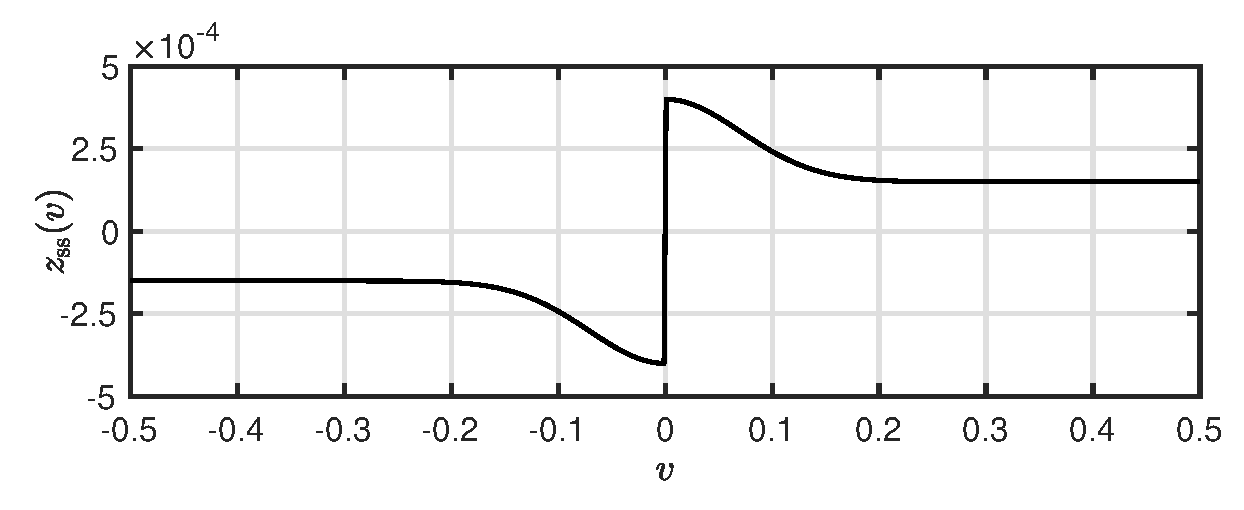
\includegraphics[width=0.8\textwidth]{figures/exciters/steadyState.eps}
    \caption{\label{fig:zss}A plot of the steady-state function $z_\text{ss}(v)$ with $s_0 = 10^4$, $\mu_\text{C} = 0.3$, $\mu_\text{S} = 0.8$, $v_\text{S} = 0.1$ and $f_\text{N} = 5$.}
\end{figure}

Finally, $\alpha(v,z)$ in Eq. \eqref{eq:zdot} is an adhesion map between the bow and the string and is defined as

\begin{equation}\label{eq:adhesionMap}
\alpha(v, z) = 
\begin{aligned}
    \begin{cases}
    \begin{rightcases}
        &0 & |z| \leq z_\text{ba}\\
        &\alpha_\text{m}(v,z)&\ \ \ \, z_\text{ba}<|z|<|z_\text{ss}(v)|\\        &1 &|z|\geq|z_\text{ss}(v)|
        \end{rightcases} 
        
        &\text{if}\  \sgn(v)=\sgn(z)\\
        \,0&\!\,\text{if}\  \sgn(v)\neq\sgn(z),
    \end{cases}
    \end{aligned}
\end{equation}
where the transition between the elastic and plastic behaviour is defined as
\begin{equation}\label{eq:alphaM}
    \alpha_\text{m} = \frac{1}{2}\bigg[1+\sgn(z)\sin\bigg(\pi\frac{z-\sgn(z)\frac{1}{2}(|z_\text{ss}(v)|+z_\text{ba})}{|z_\text{ss}(v)|-z_\text{ba}}\bigg)\bigg],
\end{equation}
with break-away displacement $z_\text{ba} = 0.7 f_\text{C}/s_0$ \todo{so is $z_\text{ba} = z_\text{ba}(t)$} determines the value of $z$ before bristles start to break. The adhesion map is visualised in Figure \ref{fig:alphaPlot} and relates to Figure \ref{fig:elastoPlastic} as described in its caption.
\begin{figure}[ht]
    \centering
    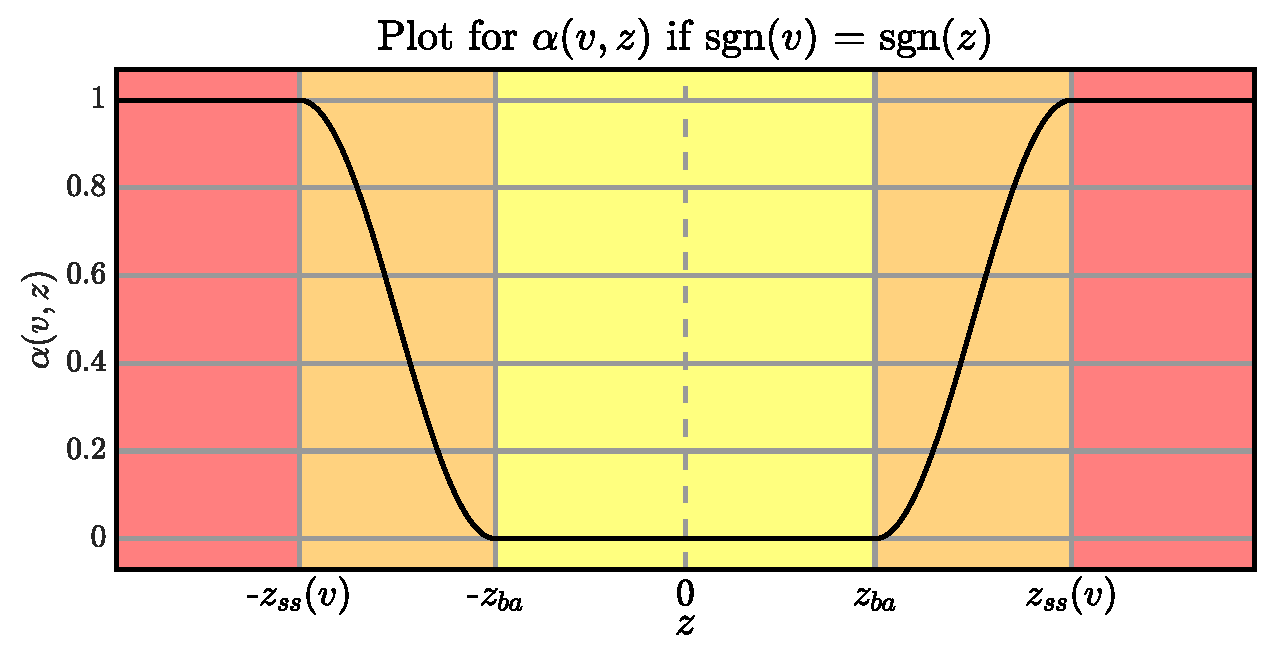
\includegraphics[width=0.8\textwidth]{figures/exciters/drawAlpha3.eps}
    \caption{\label{fig:alphaPlot}A plot of the adhesion map $\alpha(v,z)$ plotted against $z$ when the signs of $v$ and $z$ are the same. The different regions of the map are shown with the coloured areas and correspond to Figure \ref{fig:elastoPlastic} according to: yellow - a) \& b), orange - c) and red - d). (Adapted from paper \citeP[C])}
\end{figure}

\subsubsection{Discrete time}
Equation \eqref{eq:elastoPlasticForce} can be discretised to
\begin{equation}\label{eq:discForceFunction}
    f(v^n,z^n) = s_0z^n + s_1r^n+s_2v^n+s_3w^n
\end{equation} 
where discrete relative velocity in Eq. \eqref{eq:vrelElasto}
\begin{equation}
    v^n = I(x_\Btxt^n)\dtd\uln - v_\Btxt^n,
\end{equation}
and 
\begin{equation}\label{eq:r}
    r^n = r(v^n,z^n) = v^n\bigg[1-\alpha(v^n,z^n)\frac{z^n}{z_\text{ss}(v^n)}\bigg]
\end{equation}
is the discrete counterpart of \eqref{eq:zdot}. The discrete adhesion map is identical to the continuous definition given in Eqs. \eqref{eq:adhesionMap} and \eqref{eq:alphaM}, but with superscripts $n$ added for appearances of $v$ and $z$.

\subsection{Applied to a FDTD stiff string}
\SWcomment[The first appearance contribution of the PhD project in this dissertation]

In the same way as done with the static friction model in Section \ref{sec:staticFricMod}, one can add the friction force to the stiff string PDE in Eq. \eqref{eq:stiffStringPDE} and discretise the system as follows:
%
\begin{equation}\label{eq:elastoStiffStringFDS}
    \dtt \uln = c^2 \dxx \uln - \kappa^2 \dxxxx \uln - 2 \sz \dtd \uln + 2 \so\dtm\dxx \uln - J(x_\Btxt^n)\frac{f(v^n,z^n)}{\rho A}.
\end{equation}
After taking an inner product with $J(x_\Btxt^n)$ and using identities \eqref{eq:identityIJ} and \eqref{eq:identity1}, one can rewrite this similarly to the static friction model in Eq. \eqref{eq:staticFrictionNRfunc} as

\begin{equation}
    g_1(v^n,z^n) = \left(\frac{2}{k} + 2\sz\right)v^n + \lVert J(x_\Btxt^n)\rVert_\D^2\frac{f(v^n,z^n)}{\rho A}+ b^n= 0,
\end{equation}
where
\begin{align*}
    b^n =&-\frac{2}{k}I(x_\text{B}^n)\delta_{t-}u_l^n - c^2 I(x_\text{B}^n)\delta_{xx} u_l^n +\kappa^2I(x_\text{B}^n)\delta_{xxxx} u_l^n\\
    &+\left(\frac{2}{k}+ 2\sigma_0\right)v_\text{B}^n-2\sigma_1I(x_\text{B}^n)\delta_{t-}\delta_{xx}u_l^n
\end{align*}
The main issue is now is that there are two unknown variables $v^n$ and $z^n$ that part of the nonlinear function $f$. 


\subsection{Stability through Energy Analysis}
As the system at hand is nonlinear, frequency domain analysis as described in Section \ref{sec:stabilityAnalysis} can not be performed. Energy analysis, on the other hand, can be used to determine the necessary stability condition for this model. 

This section will show a necessary sta
